% !TeX root = ../../Parte2.tex
\secmeme{css/misure}
\section{Dimensioni}

\begin{frame}{Box model}\transfade\centering
  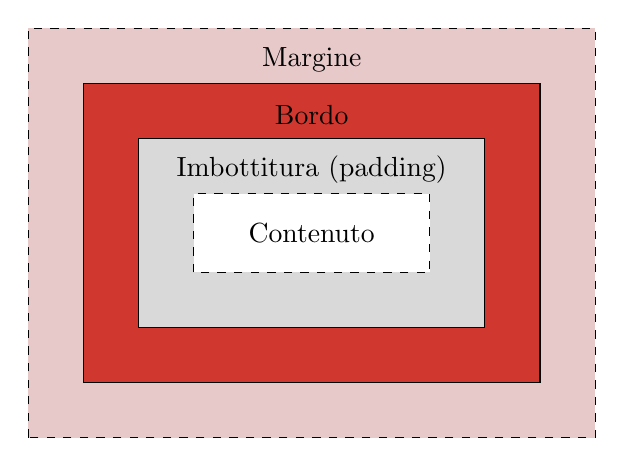
\begin{tikzpicture}

    \draw[fill=red!40!gray!30!white, dashed] (-3.6,-2.6) rectangle (3.6,2.6);
    \draw[fill=brown!20!red!70!gray] (-2.9,-1.9) rectangle (2.9,1.9);
    \draw[fill=gray!30!white] (-2.2,-1.2) rectangle (2.2,1.2);
    \draw[fill=white, dashed] (-1.5,-.5) rectangle (1.5,.5);

    \draw (0,2.2) node {Margine};
    \draw (0,1.5) node {Bordo};
    \draw (0,.8) node {Imbottitura (padding)};
    \draw (0,0) node {Contenuto};

  \end{tikzpicture}\\
\end{frame}

\begin{frame}[fragile]{Dimensione contenuto}\transfade\centering
  \begin{minted}[firstline=2, lastline=9, fontsize=\normalsize]{css}
p{
    width: 100px;
    height: auto;

    min-width: 100%;
    min-height: 100pt;

    max-width: 100px;
    max-height: 100px;
}
  \end{minted}
\end{frame}
\begin{frame}[fragile]{Bordo}\transfade\centering
  \htmlDual[-s A7][][trim={0 7cm 0 0},clip][css]{<style>}{
  p.solid {border-style: solid;}
  p.dotted {border-style: dotted;}
  p.dashed {border-style: dashed;}
  p.double {border-style: double;}
  p.none {border-style: none;}
  p.hidden {border-style: hidden;}}{
  </style>
  <p class="solid">Bordo normale.</p>
  <p class="dotted">Bordo puntinato.</p>
  <p class="dashed">Bordo trateggiato.</p>
  <p class="double">Bordo doppio.</p>
  <p class="none">Senza bordo.</p>}\pause\bigskip
  \begin{minted}[firstline=2, lastline=6, fontsize=\normalsize]{css}
    p{
border-width: 5px /*o thin, medium, thick */;
border-color: orange;
border-radius: 10px;

border: 5px solid green; /* scorciatoia */
/* border-left, border-right, border-top, border-bottom */
    }
      \end{minted}
\end{frame}

\begin{frame}[fragile]{Bordo tabelle}\transfade\centering
  \htmlDual[-s A7][][trim={0 7cm 4cm 0},clip][css]{<style>}{
  #tab1, #tab1 th, #tab1 td{
    border: 1px solid black;
  }

  #tab2, #tab2 th, #tab2 td{
    border: 1px solid black;
    border-collapse: collapse;
  }
  }{
  </style>
  <table id=tab1><tr><td>1<td>2<tr><td>3<td>4</table><br>
  <table id=tab2><tr><td>1<td>2<tr><td>3<td>4</table>}
\end{frame}

\begin{frame}[fragile]{Margine}\transfade\centering
  \htmlDual[-s A7][][trim={0 9cm 0 0},clip][css]{<style>}{
 span{
    margin: 0 20px 0 20px;
    /* equivale a:
    margin-top: 0;
    margin-right: 20px;
    margin-bottom: 0;
    margin-left: 20px;
    */
    /* margin: 0 20px; */
    border: 1px solid blue;
  }
  }{
  </style>
  <p>Lorem ipsum <span>dolor sit</span> amen.</p>}
\end{frame}

\begin{frame}[fragile]{Centrare orizzontalmente col margine auotmatico}\transfade\centering
  \htmlDual[-s A7][][trim={0 9cm 0 0},clip][css]{<style>}{
#contenitore{ /*padre*/
  border: 1px solid blue;
}
#contenuto{ /*figlio*/
  border: 1px solid orange;
  width: 200px;
  margin: auto;
}
  }{
  </style>
  <div id="contenitore"><p id="contenuto">Lorem ipsum dolor sit amen.</p></div>}
  \bigskip
  Funziona solo per i \mintcss{#contenuto} che non sono \emph{inline}.\\
\end{frame}

\begin{frame}[fragile]{Imbottitura (padding)}\transfade\centering
  \htmlDual[-s A7][][trim={0 8cm 0 0},clip][css]{<style>}{
 span{
    padding: 10px 20px 5px 15px;
    /* equivale a:
    padding-top: 10px;
    padding-right: 20px;
    padding-bottom: 5px;
    padding-left: 15px;
    */
    border: 1px solid blue;
  }
  }{
  </style><br>
  <p>Lorem ipsum <span>dolor sit</span> amen.</p>}
\end{frame}



%%%%%% MEMORY
\begin{frame}[fragile]\transfade
  \begin{exercise}\centering
    \begin{columns}
      \begin{column}{.45\textwidth}
        \htmlRender[-s A5][height=.85\textheight, trim={0 5cm 0 0},clip]{<meta charset="utf-8"><style>img{width:70px !important;height: 70px !important}</style>
    <base href="../../memory/html">
<style>
body{
    background-color: bisque;
    text-align: center;
}

h1{
    font-family: "Comic Sans MS", cursive, sans-serif;
    font-size: 40pt;
    color: blue;
}

h1, h2, h3{
    margin: 0;
}

.corretto{
    color: green;
}
.errore{
    color: red;
}

#tavolo{
    background-color: white;
    border: solid 1px black;
    border-radius: 20px;
    margin: 20px;
    padding: 15px;
}

#tavolo img{
    height: 100px;
    width: 100px;
}

footer ul a, #gioco button{
    background-color: brown;
    color: white;
    text-align: center;
    text-decoration: none;
    border: none;
    border-radius: 20px;
    padding: 10px 20px;
}
</style>
<header id="top">
    <hgroup>
        <h1> Memory </h1>
        <h2> Fai la tua mossa </h2>
    </hgroup>
</header>

<article id="gioco">
<table id="tavolo">
      <tr>
          <td><img src="img/dorso.png" alt="Dorso"></td>
          <td><img src="img/dorso.png" alt="Dorso"></td>
          <td><img src="img/dorso.png" alt="Dorso"></td>
          <td><img src="img/dorso.png" alt="Dorso"></td>
      </tr>
      <tr>
          <td><img src="img/dorso.png" alt="Dorso"></td>
          <td><img src="img/dorso.png" alt="Dorso"></td>
          <td><img src="img/dorso.png" alt="Dorso"></td>
          <td><img src="img/dorso.png" alt="Dorso"></td>
      </tr>
      <tr>
          <td><img src="img/dorso.png" alt="Dorso"></td>
          <td><img src="img/dorso.png" alt="Dorso"></td>
          <td><img src="img/dorso.png" alt="Dorso"></td>
          <td><img src="img/dorso.png" alt="Dorso"></td>
      </tr>
      <tr>
          <td><img src="img/dorso.png" alt="Dorso"></td>
          <td><img src="img/dorso.png" alt="Dorso"></td>
          <td><img src="img/dorso.png" alt="Dorso"></td>
          <td><img src="img/dorso.png" alt="Dorso"></td>
      </tr>
  </table>

<section>
<h3 class="corretto"> Giusto </h3>
<h3 class="errore"> Sbagliato </h3>
      <p> Tentativi: 0 </p>
      <p> Giuste: 0 </p>
  </section>

  <button> Ricomincia </button>
</article>

<footer>
    <ul>
        <li> <a href="https://it.wikipedia.org/wiki/Memoria_(gioco)" target="_blank"> Informazioni sul gioco </a>
        <li> <a href="#top"> Torna su </a>
    </ul>
</footer>}
      \end{column}
      \begin{column}{.45\textwidth}
        \begin{enumerate}
          \item Dimensiona le tessere a \texttt{100px}
          \item Aggiungi un bordo arrotondato al tavolo
          \item Rimuovere il margine dai titoli
          \item Aggiungi un margine di \texttt{20px} al tavolo
          \item Aggiungi un padding di \texttt{15px} al tavolo
          \item Assicurarsi che i link e i pulsanti non abbiano bordo e che siano arrotondati
          \item Aggiungi paddind ai link e pulsanti
        \end{enumerate}
      \end{column}
    \end{columns}
  \end{exercise}
\end{frame}

\begin{frame}[fragile]\transfade
  \begin{sol}\centering
    \begin{enumerate}
      \item Dimensiona le tessere a \texttt{100px}
      \makeatletter
      \inputminted[breaklines, firstline=34, lastline=37]{css}{\html@dir/\jobname _\thehtml@count.html}
      \item Aggiungi un bordo arrotondato al tavolo
      \begin{minted}{css}
#tavolo{
    border: solid 1px black;
    border-radius: 20px;
}
      \end{minted}
      \item Rimuovere il margine dai titoli
      \inputminted[breaklines, firstline=15, lastline=18]{css}{\html@dir/\jobname _\thehtml@count.html}
      \makeatother
    \end{enumerate}
  \end{sol}
\end{frame}

\begin{frame}[fragile]\transfade
  \begin{sol}\centering
    \begin{enumerate}
      \setcounter{enumi}{3}
      \item Aggiungi un margine di \texttt{20px} al tavolo
      \item Aggiungi un padding di \texttt{15px} al tavolo
      \begin{minted}{css}
#tavolo{
    margin: 20px;
    padding: 15px;
}
      \end{minted}
    \item Assicurarsi che i link e i pulsanti non abbiano bordo e che siano arrotondati
    \item Aggiungi paddind ai link e pulsanti
    \begin{minted}{css}
footer ul a, #gioco button{
    border: none;
    border-radius: 20px;
    padding: 10px 20px;
}
    \end{minted}
    \end{enumerate}
  \end{sol}
\end{frame}